\documentclass[12pt]{extarticle}
\usepackage[utf8]{inputenc}
\usepackage{cite}
\usepackage{url}
\usepackage{graphicx}
\usepackage{float}
\graphicspath{ {./figs/} }

\title{Quantification of Uncertainty in Medical Image Segmentation}
\author{Hao Wang, Yunhao Luo}
\date{December 2020}

\begin{document}

\maketitle
\begin{abstract}
Recent years have witnessed the improvement of deep learning algorithms on natural image 
analysis. However, constrained by inter-rater variability as well as short of annotations, 
the deployment of deep models into clinical practice remains a challenging problem. Though various methods
has been proposed to address the inter-rater variability, the quantification of it hasn't been 
studied extensively. Late on, a challenge named Quantification of Uncertainty in Biomedical Image Quantification(QUBIQ)
is carried out. Following the metrics given and after obtaining preliminary results, we found that a high score 
is not necessarily a good representation of inter-rater variability. Therefore, our goal is to 
further explore the inter-rater variability and to adopt a better metric for measurement of uncertainty. 
Based on that, we will be able to propose a further optimized method. 
\end{abstract}
\section{Introduction}
\paragraph{}
Recent development of deep learning algorithms has greatly improved 
the performance on natural image analysis. 
Adequate algorithms have been proposed to address image classification and semantic
segmentation problems. Large-scale datasets with abundant annotations have also been
published \cite{nair_precup_arnold_arbel_2020}.
However, due to
% inter-reader variations need more details and background
lack of annotations and high inter-rater variations\cite{zhang2020disentangling}
in medical domain, the application of deep models on clinical diagnosis,
% TODO:
known to be sensitive to false-positive and true-negative cases, is still a challenging problem.
For instance, the inter-rater variations of glioblastoma segmentation
is pointed out to be in the range of 74-84\% \cite{6975210}.
Studies on inter-rater variance also found that
inconsistency among annotations of biomedical structures widely exists
\cite{Variability2019}\cite{interobserver2018}. Such high-variant dataset 
could result in poor performance of supervised machine learning algorithms,
which are known to be highly dependent on the quality of data as well as their annotations.
To overcome it, the most straight-forward and widely-adopted method 
is to take the majority vote of experts' annotations, treating every 
experts' opinions equally significant\cite{6975210}. Another method, STAPLE, proposed by \cite{STAPLE} 
evaluates reliability of annotators and assigns weights to each of them when 
fusing annotations accordingly. However, both of the approaches focus on per image annotation fusion
while ignoring information across the whole dataset\cite{zhang2020disentangling}.
In 2020, a challenge about quantification of uncertainty 
in biomedical image segmentation has been carried
out on the purpose of seeking measures to quantify the uncertainty of 
medical image annotation. A discrete approximation of the uncertainty is also
proposed for the assessment of participants' results. It
takes in the averaged ground truth and the provided predicted probability map of a task
% TODO: explain threshold
and computes average dice score for each threshold value respectively 
\cite{qubiq}. 
A high averaged dice score is then considered to be an indication of 
good quantification of the inter-rater uncertainty.
For the first step, our goal is to follow the QUBIQ challenge and quantify 
uncertainties in biomedical image segmentation. 
However, the drawback for the QUBIQ evaluation metric is distinct: it 
ignores the fact that most uncertain pixels lie around 
the contour of the lesion area. Therefore we are expecting to have a
better evaluation method for inter-rater variations as well as an objective function for 
optimization. Finally, based on the metric, a further
optimized method could be explored.
\section{Related Works}
\paragraph{}
Uncertainty in deep learning can be divided into \textit{Aleatoric}
uncertainty and \textit{Epistemic} uncertainty \cite{kendall2017uncertainties}.
\textit{Aleatoric} uncertainty or data uncertainty typically occurs during data sampling and might be caused by 
observers and sampling devices.
Usually, it is irreducible even feeded with more data, which shares a
close connection with inter-rater variations. On the other hand, \textit{Epistemic}
uncertainty refers to ambiguity of model prediction that can be reduced by feeding abundant data.
For example, a model trained on only part of a dataset may over-confidently
predict unseen data into wrong classes. Recent research on 
Bayesian Neural Network(BNN) has made it possible to quantify the 
uncertainty of model prediction by replacing scalar parameters with probabilistic distributions. Since parameters are now sampled 
from a `pre-defined" prior distribution, 
the outputs' variance reflects the predictive uncertainty of the model and could be considered a 
combination of \textit{aleatoric} uncertainty and \textit{epistemic} uncertainty. 
Kohl et al.\cite{kohl2019probabilistic} 
proposed a method that involves uncertainties by deploying variational 
auto-encoder(VAE) into U-Net, the widely used model in medical image segmentation\cite{ronneberger2015unet}. 
The VAE here accounts for variations of annotations and represents an 
estimation of joint distribution that includes every pixels of the segmentation map. 
The framework is capable of providing multiple segmentation 
hypotheses with each of them estimating the knowledge of one expert.
Some recent studies proposed to use a dropout network as an approximation of BNN by keeping dropout at test stage. 
Predictions are sampled using Monte Carlo methods and various 
uncertainties are computed based on the sampled results.
It is also reported that effective performance can be achieved 
without any additional parameters compared with non-Bayesian methods. 
However, for such methods, the ambiguity obtained is
% Aleatoric & Epistemic uncertainty needs more explanation
not a direct representation of the \textit{Aleatoric} uncertainty(the noise of data)
, but \textit{epistemic} uncertainty in model
\cite{kendall2017uncertainties}. 
Therefore, when only insufficient data is provided, the resulted uncertainty could not
be treated as the inter-rater variability but the reliability of 
the model itself. 
\cite{nair_precup_arnold_arbel_2020}. 
\paragraph{}
Another study by \cite{zhang2020disentangling} uses confusion matrices to
model each annotator. They hold three assumptions: first, there is one and
only one ground truth annotation for an input of certain task setting; 
second, annotations are noised approximation of the ground truth;last, annotators could be modeled by confusion matrices.
Then, annotations can be estimated by matrix multiplication of annotators'
confusion matrices with ground truth. The framework has two convolution neural network backbone
where one outputs the estimated ground truth and the other accounts for the confusion matrices
of each annotator. 
A unique ground truth could be learned by minimizing the 
cross entropy of the matrix multiplication result and the real annotation.
Though the inter-rater variance is not directly measured, the well-modeled annotators'
confusion matrices could be utilized to produce further results
as well as measurements of uncertainties.
Nevertheless, the correctness of the assumption of this approach
still remains to be verified since there's no dataset available 
that fulfils their requirement by the publish time of their work.
\paragraph{}
To accurately model the inter-rater variability, Hu et al.\cite{hu2019supervised} utilized a multiple annotator dataset
to produce a `ground truth" for \textit{Aleatoric} uncertainty. Then a supervised framework for estimating
as well as quantifying \textit{Aleatoric} uncertain is proposed and combined with probabilistic U-Net
to produce fine-grained uncertainty approximations. 

\section{Method}
\begin{figure}[hb!]
\centering
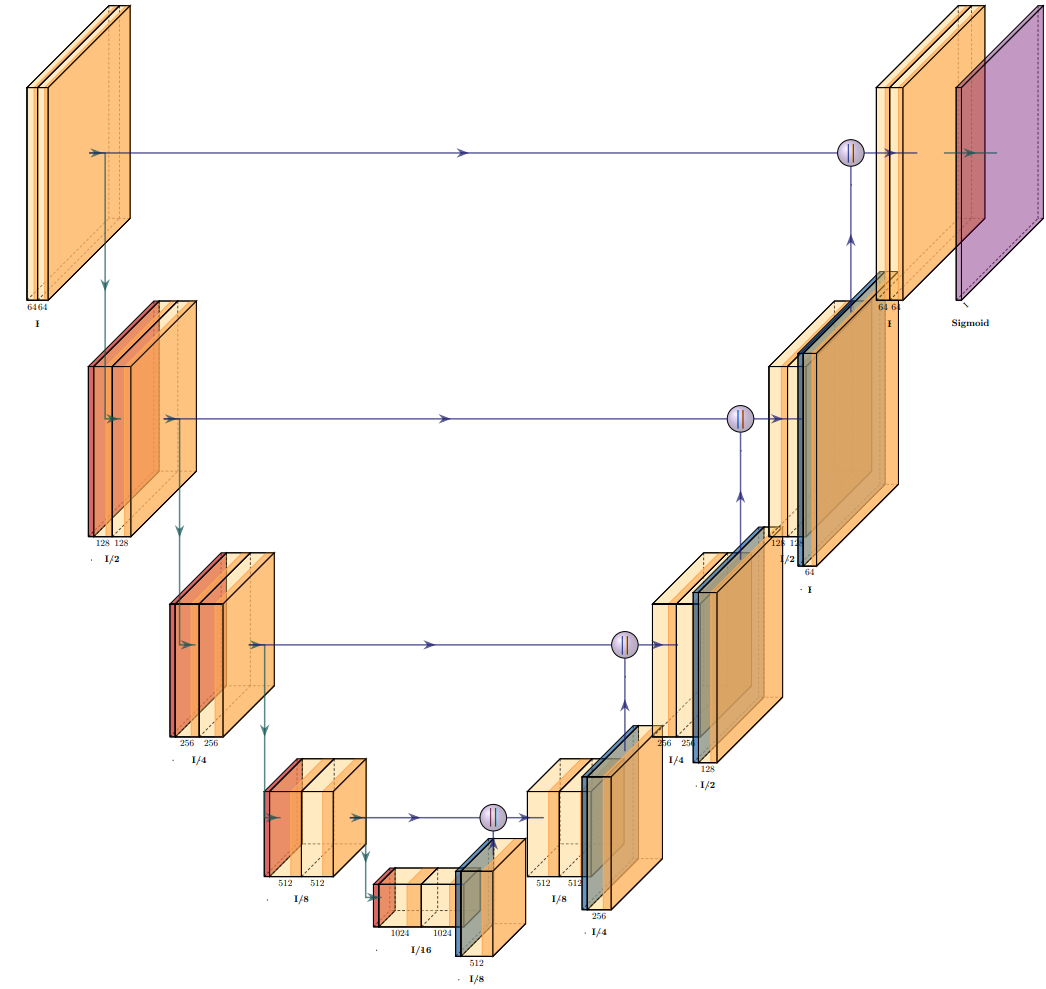
\includegraphics[scale=0.28]{fig2.png}
\caption{U-Net architecture\cite{iqbal_2018}}
\label{pre_results}
\end{figure}
\begin{figure}[ht!]
\centering
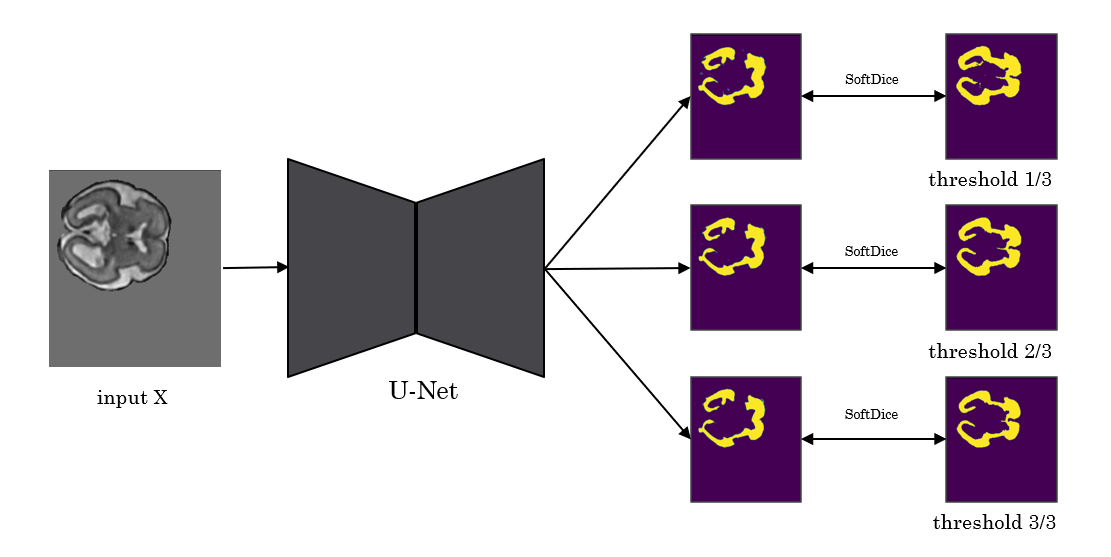
\includegraphics[scale=0.3]{fig3.png}
\caption{Our baseline method}
\label{proposed_mothod}
\end{figure}
\begin{figure}[ht!]
\centering
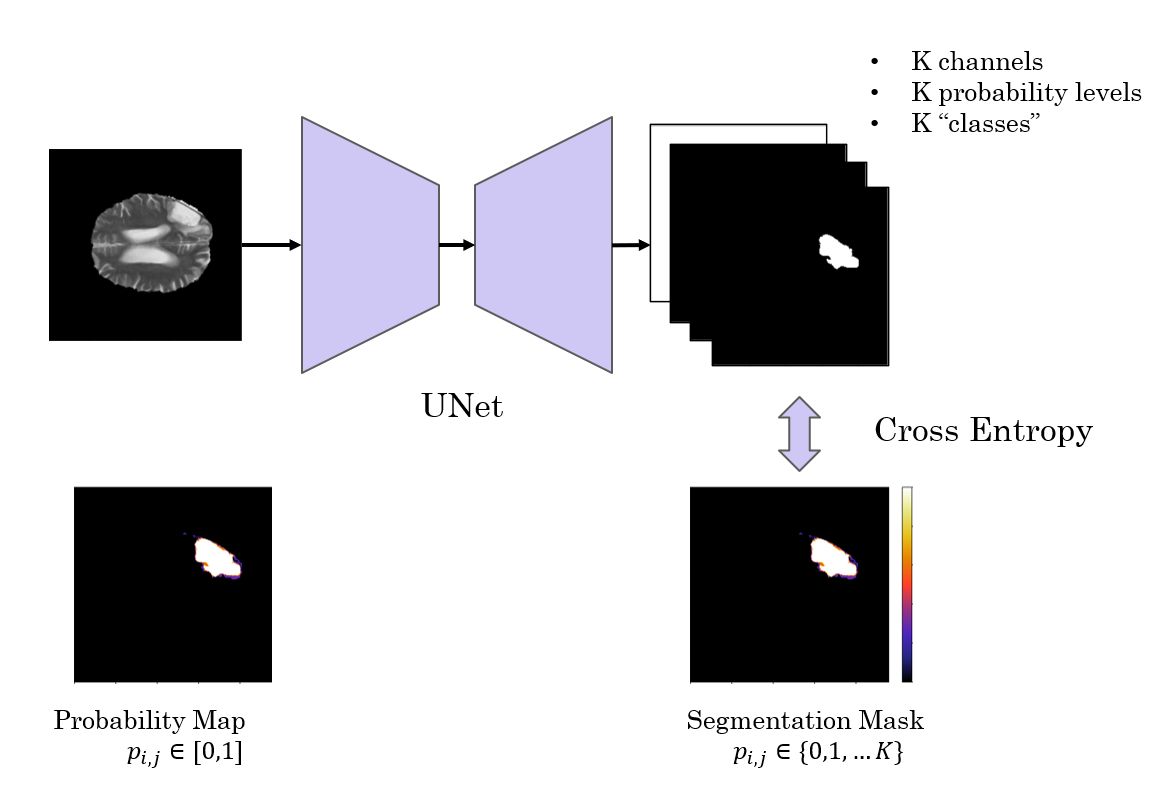
\includegraphics[scale=0.3]{fig6.png}
\caption{Second Design: Using \textit{CrossEntropy} as objective function. Reformulate the problem as multi-class segmentation}
\label{leveling}
\end{figure}
\paragraph{}
To model the inter-rater variability in the segmentation task, 
we follow the metric given by \cite{qubiq} and estimate the threshold binary map at each probability level.
of $\frac{1}{M}, \frac{2}{M}, ..., \frac{M}{M}$, 
where $M$ is the number of annotators. It could be considered as the discrete cumulative distribution of 
the uncertainty caused by inter-rater variability. Cumulative, which includes more information can 
provide more context for estimation of uncertainty. A preliminary result is obtained and  
shown in section 4 using this method and U-Net as backbone model.
\begin{equation}
    y_{p} = \{y_{p\frac{1}{M}}, y_{p\frac{2}{M}}, ... y_{p\frac{M-1}{M}},y_{p\frac{M}{M}}\}
\end{equation}
\begin{equation}
    y_{g} = \{y_{g\frac{1}{M}}, y_{g\frac{2}{M}}, ... y_{g\frac{M-1}{M}},y_{g\frac{M}{M}}\}
\end{equation}
\begin{equation}
    L = 1 - \frac{1}{NM}\sum_{n=1}^{N}\sum_{m=1}^{M}SoftDice(y_{p\frac{m}{M}}^{(n)}, y_{g\frac{m}{M}}^{(n)})
\end{equation}
\begin{equation}
    SoftDice(y_p, y_g) = \frac{2\sum y_p y_g}{\sum y_p +  \sum y_g + \epsilon}
\end{equation}
where $y_p$ is the prediction with each
channel representing an estimation of binary segmentation map at multiple threshold values, 
$y_g$ the ground truth binary segmentation map with corresponding threshold 
values as $y_p$ and $\epsilon$ is the smooth factor that smooths 
the training process by avoiding fluctuation caused by division of small value.
$L$ is the loss function that maximizes the similarity 
between $y_p$ and $y_g$ using soft dice coefficient 
to be optimized with stochastic gradient descend. 
\begin{figure}[ht!]
\centering
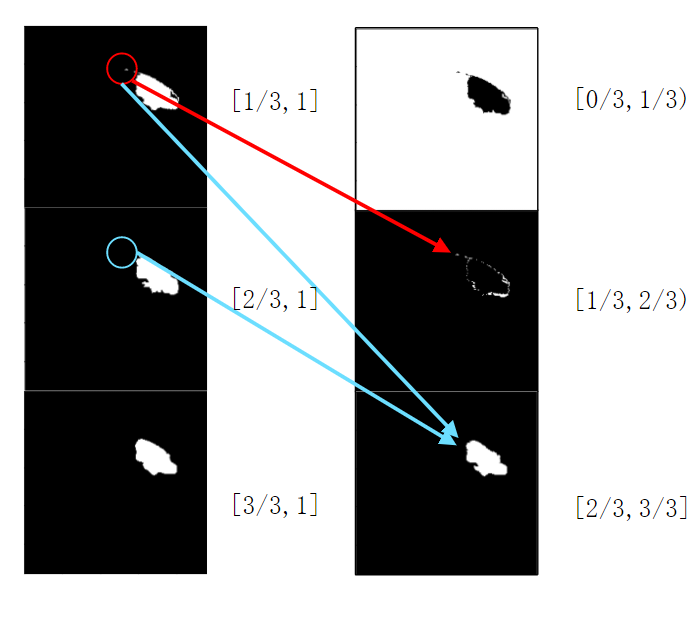
\includegraphics[scale=0.3]{fig7.png}
\caption{Wrongly predicted pixels affect final result}
\label{WrongResult}
\end{figure}
\paragraph{}
However, since during training, no extra constrained is applied on inter-channel relations, the result could be 
affected and unstable according to Figure.\ref{WrongResult}. To be more discriminative, we can reformulated the 
problem as a multi-class segmentation problem, with each probability level as a class. Then, \textit{CrossEntropy} can 
be used as the proxy objective function for optimization. The architecture is shown in Figure.\ref{leveling}
\paragraph{}
To further imporve the performance of our method, we combine the above mentioned methods in a unified framework, named as Threshold\&Leveling.
Computing threshold result based on single probability is not feasible requires a step function like activation function.

\section{Results and Analysis}
\begin{figure}[ht!]
\begin{center}
    \begin{tabular}{|| c | c | c | c ||}
       \hline
       Task Number & Threshold & Leveling & Threshold \& Leveling \\
       \hline \hline
        Brain-tumor Task 1 & 0.818 & \textbf{0.828} & 0.826 \\
        Brain-tumor Task 2 & 0.847 & 0.869 & \textbf{0.922}\\
        Brain-tumor Task 3 & \textbf{0.862} & 0.854 & \textbf{0.862}\\
        Kidney & \textbf{0.811} & 0.783 & 0.783\\
        Brain-growth & 0.509 & \textbf{0.542} & 0.500  \\
        Prostate 1 & 0.512 & \textbf{0.574} & 0.561 \\
        Prostate 2 & 0.554 & \textbf{0.570} & 0.563\\
        \hline \hline
    \end{tabular}
\end{center}
\caption{Mean dice score under QUBIQ evaluation metric}
\end{figure}
\paragraph{}
This part we demonstrate our results obtained on the QUBIQ uncertainty dataset.
The result shown in Figure \ref{pre_results} is obtained using the method mentioned in the previous 
section without pre-training nor data augmentation.
Though it could be considered a medium-level result for a segmentation task, especially for such
a small amount of data samples, as for uncertainty, most of the uncertain pixels around the contour area are not 
correctly approximated. It's a reflection of the weakness of the objective of 
being not focused enough on uncertain data point or could be considered a high \textit{epistemic} uncertainty. 
Larger weights should be assigned to those pixels with high inter-rater variability. Pre-training on 
related single annotator dataset may also help reduce the difference between 
prediction and ground truth \textit{aleatoric} uncertainty.
\paragraph{}
Since for task brain-tumor and kidney, there's only 3 annotators available, the advantage of \textit{CrossEntropy} as 
multi-class objective function becomes less obvious. However, for Brain-growth and Prostate with more that 6 annotators, \textit{CrossEntropy}
wins a large margin over threshold and channels-wise dice loss. Judging from the characteristics of two type of 
loss function, the results are reasonable since CrossEntropy loss assign equal weights to each probability level after reweighting while 
DiceCoef loss focuses on the lesion area. 
\paragraph{}
The combined method mananged to imporve the performance on tasks with less annotations, which outcompetes the leveling method and also has 
an edge over the threshold method. However, it fails to improve the performance on datasets with 
more annotations for each image. The reason could be that threshold in the combined method puts extra 
weights on the central parts which are more important for tasks with les annotations but becomes insignificant when
the number of annotations per image increases. As a result, the extra supervised signal brought about by threshold 
is not as effective as expected.
\section{Evaluation Metrics}
\paragraph{}
Based on the metric provided by \cite{qubiq}, a naive evaluation of our result could be given by:
\begin{equation}
    S = \frac{1}{TNH}\sum_{t=1}^{T}\sum_{n=1}^{N}\sum_{h=1}^{H}DiceCoef(y_{p\frac{h}{H}}^{(t)}, y_{g\frac{h}{H}}^{(t)})
\end{equation}
where T is total number of tasks, N is the size of the validation set and H refers to 
the number of threshold values. It could be considered a discrete estimation of quality of the cumulative probability 
distribution.
\paragraph{}
To further explore the quality \textit{aleatoric} uncertainty as well as the accuracy and sample diversity, we plan to 
adopt the generalized energy distance metric, that has the form:
\begin{equation}
    D^2_{GED} = 2E[d(S, Y)] - E[d[S, S']] - E[d(Y, Y')]
\end{equation}
\begin{equation}
    d(A, B) = 1 - IoU(A, B)
\end{equation}
where S is samples from the bayesian model or Monte Carlo dropout model, Y is the corresponding 
annotations. The first term of GED accounts for the difference between sampled predictions
and annotations. The rest terms quantify the expected difference of the sampled predictions and 
annotations among themselves. 

% TODO
% Problem Formulation
% \begin{enumerate}
%    \item Achieve high performance under QUBIQ evaluation metrics.
%    \item Define a better metric for the assessment of uncertainties in medical image segmentation.
%    \item Derive a method for the measurement of data uncertainties.
%    \item Address uncertainties caused by inter-reader variations.
%\end{enumerate}

\bibliographystyle{plain}
\bibliography{M335}

\end{document}
